\documentclass{standalone}
\usepackage{pgfplots}
%\usepackage{fontspec}
\usetikzlibrary{arrows,positioning}

\renewcommand{\familydefault}{\sfdefault}

\begin{document}

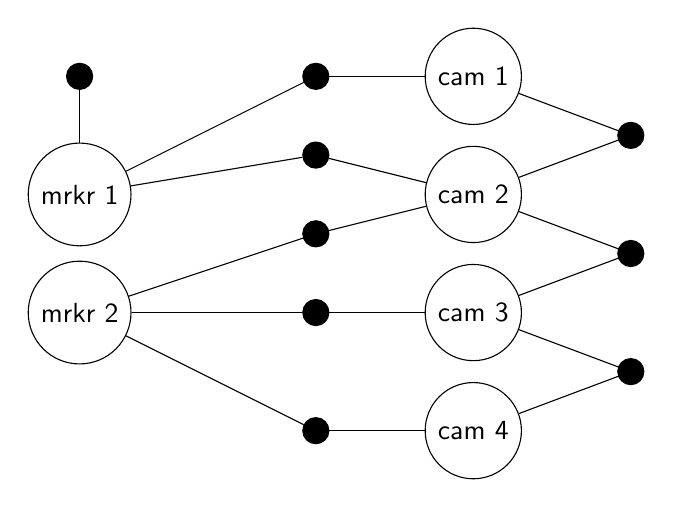
\begin{tikzpicture}[auto,decoration={random steps,segment length=1mm,amplitude=0.3pt},
  factor/.style={draw,circle,minimum size=0.2cm,fill=black},
  state/.style={draw,circle,align=center}]


\foreach \x in {1,...,2}
{
  \node[state] (mkr\x) at (0, 4.5 - 1.5*\x) {mrkr \x};
}
  
\node[factor] (prior) at (0, 4.5) {};
\path (prior) edge (mkr1);

\foreach \x in {1,2,3,4}
{
  \node[state] (cam\x) at (5, 6-1.5*\x) {cam \x};
}

\foreach \x in {1,3,4}
{
  \node[factor] (meas\x) at (3, 6-1.5*\x) {};
  \path[-] (cam\x) edge (meas\x);
}

\node[factor] (meas2a) at (3, 3.5) {};
\node[factor] (meas2b) at (3, 2.5) {};
\path (cam2) edge (meas2a);
\path (cam2) edge (meas2b);

\path (mkr1) edge (meas1);

\path (mkr1) edge (meas2a);
\path (mkr2) edge (meas2b);

\path (mkr2) edge (meas3);

\path (mkr2) edge (meas4);

\foreach \x in {1,...,3}
{
  \pgfmathtruncatemacro{\y}{\x+1}
  \node[factor] (between\x) at (7, 5.25-1.5*\x) {};
  \path (cam\x) edge (between\x);
  \path (cam\y) edge (between\x);
}


\end{tikzpicture}

\end{document}
